\chapterA{Modelado}
\section{Introducción}
La fase de modelado es la segunda etapa del proceso de Diseño Guiado por Objetivos (DGO). En esta fase, partiremos de la lista de factoides que
obtuvimos en la etapa anterior y con ella diseñar los prototipos de personas que serán los potenciales usuarios de la misma, representando además
las principales características que extrajimos de los factoides.

Para poder lograr este objetivo, tenemos que realizar una serie de pasos, que van a ser los siguientes:
\begin{itemize}
    \item \textbf{Identificación de variables de comportamiento} $\rightarrow$ El primer paso que vamos a seguir es identificar las distintas variables de comportamiento que vamos a tener en la lista de factoides y ver los posibles valores que van a tomar.
    \item \textbf{Relación de individuos con las variables de comportamiento} $\rightarrow$ Tras haber identificado las variables, vamos a ver para cada uno de los usuarios entrevistados el valor que van a tomar cada una de ellas en base a los factoides obtenidos.
    \item \textbf{Identificación de patrones de comportamiento} 
\end{itemize}

\section{Planificación del hito}
Para poder planificar este hito correctamente, hemos identificado en una Hoja de cálculo (ver figura \ref{fig:planif-hito2}) las distintas tareas que tenemos que 
realizar, junto al intervalo de fechas en el que se encuentra prevista su realización y el / los responsables de dicha tarea.
\begin{figure}[H]
    \centering 
    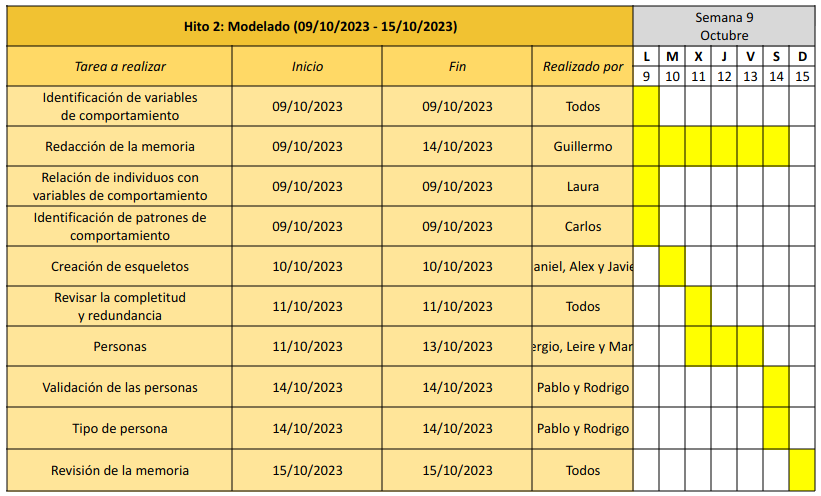
\includegraphics[width=0.8\textwidth]{./Imagenes/Planificaciones/Planif-hito2.png}
    \caption{Planificación Hito 2}
    \label{fig:planif-hito2}
\end{figure}

\section{Identificación de variables de comportamiento}
\section{Relación de individuos con variables de comportamiento}
Tras haber identificado las variables de comportamiento en la fase anterior, vamos a ver para cada uno de los usuarios entrevistados (en base a los factoides
que tenemos registrados) los valores que van a tomar en cada una de ellas. Para mostrar estos resultados vamos a realizar una matriz (ver cuadro \ref{table:relacion-individuos-variables})
en la que vamos a enfrentar cada una de las variables con los entrevistados, poniendo en cada celda el valor que va a tomar la variable para dicho usuario.
\begin{table}[H]
    \centering
    \begin{tabular}{p{10em}|p{7em}|p{7em}|p{7em}|p{8em}|}
        \cline{2-5}
                                          & Madi        & Sofía                          & Alberto            & Beatriz                         \\ \hline
        Rango de edad                     &             & 18 - 25                        & 18 - 25            & 18 - 25                         \\ \hline
        Estado civil                      & Si          & Soltera                        & En pareja          & En pareja                       \\ \hline
        Organización de viajes            & Si          & Si                             & Si                 & Si                              \\ \hline
        Uso de comparadores de viajes     & No          & Kayak, Skyscanner, Trivago     & No                 & eDreams, comparador de Google   \\ \hline
        Frecuencia de viaje               & Baja        & Media                          & Alta               & Baja                            \\ \hline
        Tipo de viaje                     & Trabajo     & Ocio                           & Ocio               & Ocio                            \\ \hline
        Discapacidad                      & No          & No                             & No                 & No                              \\ \hline
        Acompañante                       &             & Familia                        & Pareja             & Familia                         \\ \hline
        Medio de transporte más frecuente & Tren        & Transporte público             & Vehículo propio    & Vehículo propio                 \\ \hline
        Uso de tecnología                 &             & Alto                           & Alto               & Alto                            \\ \hline
        Viaje nacional                    & Si          & Si                             & Si                 & Si                              \\ \hline
        Viaje internacional               & Si          & Si                             &                    & Si                              \\ \hline
        Trabaja                           & Si          & No                             & Si                 & No                              \\ \hline
        Gusto por viajar                  &             & Si                             & Si                 & Si                              \\ \hline
        Nivel de ahorro                   & Alto        & Alto                           & Medio              & Alto                            \\ \hline
    \end{tabular}
    \caption{Tabla de relación de los individuos con las variables de comportamiento}
    \label{table:relacion-individuos-variables}
\end{table}

Una vez construida la matriz que relaciona los individuos con las variables, vamos a justificar las razones por las cuáles hemos asignado un
determinado valor a las variables para cada uno de los usuarios. \\

\noindent Justificación de las variables de Madi:
\begin{itemize}
    \item \textbf{Rango de edad} $\rightarrow$ No lo ha comentado.
    \item \textbf{Estado civil} $\rightarrow$ No lo ha comentado.
    \item \textbf{Organización de viajes} (Si) $\rightarrow$ “Madi se encarga de organizar los viajes cuadrando horarios y comprando billetes.”
    \item \textbf{Uso de comparadores de viajes} (No) $\rightarrow$ “Madi no utiliza comparadores porque ya tiene localizadas dos compañías y Renfe que ofrecen el servicio de acompañamiento de AENA.”
    \item \textbf{Frecuencia de viaje} (Alta) $\rightarrow$ “Madi se encarga de los viajes de campeonatos internacionales que ella les recepciona, les recoge y les lleva al punto de encuentro. Madi comenta que hay bastantes campeonatos.” Porque al menos asiste a los viajes internacionales que pueden ser no muy frecuentes.
    \item \textbf{Tipo de viaje} (Trabajo) $\rightarrow$ Se encarga de los viajes de su trabajo y viaja por ello.
    \item \textbf{Discapacidad} (No) $\rightarrow$ Se deduce porque trabaja en una federación y organiza viajes para gente con discapacidad.
    \item \textbf{Acompañante} $\rightarrow$ No lo ha comentado, podría ser sus compañeros de trabajo.
    \item \textbf{Medio de transporte más frecuente} $\rightarrow$ no se sabe realmente, podría ser avión o tren.
    \item \textbf{Uso de la tecnología} $\rightarrow$ tampoco lo comenta, sólo el de los deportistas.
    \item \textbf{Viaje Nacional} (Si) $\rightarrow$ “Madi comenta que en los campeonatos de españa, los clubes son los encargados del desplazamiento de los deportistas, ella interviene poco o nada.” eso significa que el poco puede llegar a viajar en algún momento en los nacionales.
    \item \textbf{Viaje internacional} (Si) $\rightarrow$ “Madi se encarga de los viajes de campeonatos internacionales que ella les recepciona, les recoge y les lleva al punto de encuentro. Madi comenta que hay bastantes campeonatos.”, recoge a los deportistas por lo que hace el viaje.
    \item \textbf{Trabaja} (Si) $\rightarrow$ “Madi es secretaria de la FEDDI y lleva 16 años trabajando allí.”
    \item \textbf{Gusto por viajar} $\rightarrow$ No lo ha dicho.
    \item \textbf{Nivel de Ahorro} (Alto) $\rightarrow$ “Madi compra billetes a través de Renfe, Air Europa o Iberia porque le sale más económico que en un comparador.” suponemos que escoge lo más económico para ahorrar lo máximo posible.
\end{itemize}

\noindent Justificación de las variables de Sofía:
\begin{itemize}
    \item \textbf{Rango de edad} (18 - 25) $\rightarrow$ “Sofía tiene 21 años.”
    \item \textbf{Estado civil} (Soltero) $\rightarrow$ No lo ha comentado, pero parece no tener pareja. 
    \item \textbf{Organización de viajes} (Si) $\rightarrow$ “Sofía a veces organiza los viajes que hace y a veces no.”
    \item \textbf{Uso de comparadores de viajes} (Kayak, Skyscanner, Trivago) $\rightarrow$ “Sofía utiliza varios comparadores de viajes a la hora de organizar un viaje. Por ejemplo: Kayak, Skyscanner, Trivago.”
    \item \textbf{Frecuencia de viaje} (Media) $\rightarrow$ “Sofía viaja a menudo, tanto fuera como dentro de España.”, a menudo será lo normal.
    \item \textbf{Tipo de viaje} (Ocio) $\rightarrow$ “Sofía ha hecho viajes de varios tipos. Desde intercambios lingüísticos a viajes familiares o con amigos, para conocer nuevas ciudades o relajarse.”
    \item \textbf{Discapacidad} (No) $\rightarrow$ “Sofía considera que los comparadores de viajes son bastante accesibles, pero que quizás aclarar algunas cosas en las webs o los anuncios de spam en las webs pueden molestar a personas con discapacidad intelectual.” da a intuir que ella no tiene discapacidad.
    \item \textbf{Acompañante} (Familia) $\rightarrow$ “A Sofía le gusta ir alternando entre viajar sola, con familia o con amigos, disfruta de todas.” Más con familia ya que es estudiante y no tiene trabajo para pagar tantos viajes.
    \item \textbf{Medio de transporte más frecuente} (Transporte público) $\rightarrow$ “Sofía usa tanto automóviles como trenes y autobuses en sus viajes dependiendo del sitio al que viaje.” “Sofía prefiere usar autobuses solo cuando viaje distancias cortas o medias” En cualquiera de los dos casos incluye transporte público.
    \item \textbf{Uso de la tecnología} (Alto) $\rightarrow$ “Sofía tiene 21 años y considera que tiene un buen manejo de la tecnología”
    \item \textbf{Viaje Nacional} (Si) $\rightarrow$ “Sofía viaja a menudo, tanto fuera como dentro de España.”
    \item \textbf{Viaje internacional} (Si) $\rightarrow$ “Sofía viaja a menudo, tanto fuera como dentro de España.”
    \item \textbf{Trabaja} (No) $\rightarrow$ “Sofía es estudiante, tiene 21 años y considera que tiene un buen manejo de la tecnología” 
    \item \textbf{Gusto por viajar} (Si) $\rightarrow$ “A Sofía le gusta viajar y desde pequeña ha querido conocer las diferentes partes del mundo.”
    \item \textbf{Nivel de Ahorro} (Alto) $\rightarrow$ “Sofía busca viajes económicamente accesibles.” quiere ahorrar lo máximo posible.
\end{itemize}

\noindent Justificación de las variables de Alberto:
\begin{itemize}
    \item \textbf{Rango de edad} (18 - 25) $\rightarrow$“Alberto tiene 22 años y es informático.”
    \item \textbf{Estado civil} (En Pareja) $\rightarrow$ “Alberto suele viajar con su pareja.”
    \item \textbf{Organización de viajes} (Si) $\rightarrow$ “Alberto prepara o busca un itinerario antes de viajar, incluso toma apuntes de paradas por si le falla el móvil o gps, le parece tedioso igualmente y se encarga con su pareja.”
    \item \textbf{Uso de comparadores de viajes} (No) $\rightarrow$ “Alberto sólo usa comparadores para alojamientos mirando lo visual que sea, la localización y el precio.” sólo usa comparadores de alojamiento y no de viajes.
    \item \textbf{Frecuencia de viaje} (Alta) $\rightarrow$ “Alberto viaja una vez al mes.”
    \item \textbf{Tipo de viaje} (Ocio) $\rightarrow$ “Alberto viaja exclusivamente por ocio.”
    \item \textbf{Discapacidad} (No) $\rightarrow$ “Alberto no tiene discapacidad.”
    \item \textbf{Acompañante} (Pareja) $\rightarrow$ “Alberto suele viajar con su pareja.”
    \item \textbf{Medio de transporte más frecuente} (Vehículo propio) $\rightarrow$ “Alberto usa normalmente vehículo propio para viajar.”
    \item \textbf{Uso de la tecnología} (Alto) $\rightarrow$ “Alberto se desenvuelve bien con las tecnologías y le parecen fáciles de usar.”
    \item \textbf{Viaje Nacional} (Si) $\rightarrow$ “Prefieren conocer la península por ahora” y como comentó “Alberto viaja una vez al mes.” pues se deduce que viaja a nivel nacional sólo.
    \item \textbf{Viaje internacional} $\rightarrow$ Le gustaría viajar pero no ha comentado si ha viajado.
    \item \textbf{Trabaja} (Si) $\rightarrow$ “Alberto tiene 22 años y es informático.”
    \item \textbf{Gusto por viajar} (Si) $\rightarrow$ “A Alberto le gusta viajar para descubrir historias, paisajes y nuevas culturas.”
    \item \textbf{Nivel de Ahorro} (Medio) $\rightarrow$ “Alberto sólo usa comparadores para alojamientos mirando lo visual que sea, la localización y el precio.” estaría dispuesto a pagar más para que se cumplan los otros requisitos.
\end{itemize}

\noindent Justificación de las variables de Beatriz:
\begin{itemize}
    \item \textbf{Rango de edad} (18 - 25) $\rightarrow$ “Beatriz tiene 21 años.”
    \item \textbf{Estado civil} (En pareja) $\rightarrow$ "Va a viajar a ver a su pareja en los próximos meses".
    \item \textbf{Organización de viajes} (Si) $\rightarrow$ “Cuando no viaja con su familia, Beatriz suele organizar los viajes que hace. Cuando va con su familia, lo organiza todo el núcleo familiar en conjunto”.
    \item \textbf{Uso de comparadores de viajes} (eDreams, comparador de Google)
    \item \textbf{Frecuencia de viaje} (Baja) $\rightarrow$ “Beatriz viaja una vez al año, sobre todo dentro de España, y fuera de España una vez cada dos años.” es poco
    \item \textbf{Tipo de viaje} (Ocio) $\rightarrow$ “Beatriz suele viajar para visitar a familiares o por razones de ocio.”
    \item \textbf{Discapacidad} $\rightarrow$ No lo dice en ningún momento.
    \item \textbf{Acompañante} (Familia) $\rightarrow$ “Beatriz suele viajar acompañada, mayoritariamente por algún familiar suyo”.
    \item \textbf{Medio de transporte más frecuente} (Vehículo propio) $\rightarrow$ “Suele viajar en coche o en avión para distancias más largas.” como es dentro de España lo más normal, viaja en vehículo propio más frecuentemente.
    \item \textbf{Uso de la tecnología} (Alto) $\rightarrow$ “Beatriz se desenvuelve bien con las tecnologías y declara usarlas a diario.”
    \item \textbf{Viaje Nacional} (Si) $\rightarrow$ “Beatriz viaja una vez al año, sobre todo dentro de España, y fuera de España una vez cada dos años.”
    \item \textbf{Viaje internacional} (Si) $\rightarrow$ “Beatriz viaja una vez al año, sobre todo dentro de España, y fuera de España una vez cada dos años.”
    \item \textbf{Trabaja} $\rightarrow$ No lo comenta
    \item \textbf{Gusto por viajar} (Si) $\rightarrow$ “A Beatriz le gusta viajar para conocer otros lugares y culturas.”
    \item \textbf{Nivel de Ahorro} (Alto) $\rightarrow$ “Para Beatriz no es ningún problema sacrificar algunas facilidades como el  tipo y la cantidad de equipaje que se puede llevar, el hecho de elegir asiento o los horarios de ida y vuelta porque cuanto más barato mejor.”
\end{itemize}

\section{Identificación de patrones de comportamiento}
Tras realizar el análisis de la matriz anterior hemos identificado los siguientes patrones de comportamiento:
\begin{itemize}
    \item La gente entre 18 y 25 años comparte un gusto por viajar y sobre todo viajes de ocio.
    \item La gente entre 18 y 25 años joven tiene un alto uso de la tecnología.
    \item Todos organizan viajes y casi todos tienen un nivel de ahorro alto. 
    \item La gente entre 18 y 25 años comparte el gusto por viajar.
    \item La mitad de las personas utilizan comparadores para organizar los viajes.
    \item La mitad de la gente entrevistada viaja con sus familiares.
    \item A casi todos los entrevistados les gustan los viajes internacionales.
    \item En general la frecuencia de viajes de los usuarios son media-bajas.
\end{itemize}

Vamos a tener dos tipos de personas. Personas que viajen por ocio, en general jóvenes, que se organicen sus propios viajes con un gusto por viajar. Y por otro lado tendremos otro tipo de personas que trabajen y que viajen por trabajo y estas personas no utilizan comparadores de viajes.

\section{Creación de esqueletos}
\section{Revisar la completitud y la redundancia}
\section{Personas}
\section{Validación de las personas}
\section{Tipos de personas}